\chapterimage{head2.png} % Chapter heading image
\chapter{\normalsize Stable Diffusion vs Stable Diffusion XL}
\section*{Stable Diffusion}


\begin{figure}[H]
    \centering
    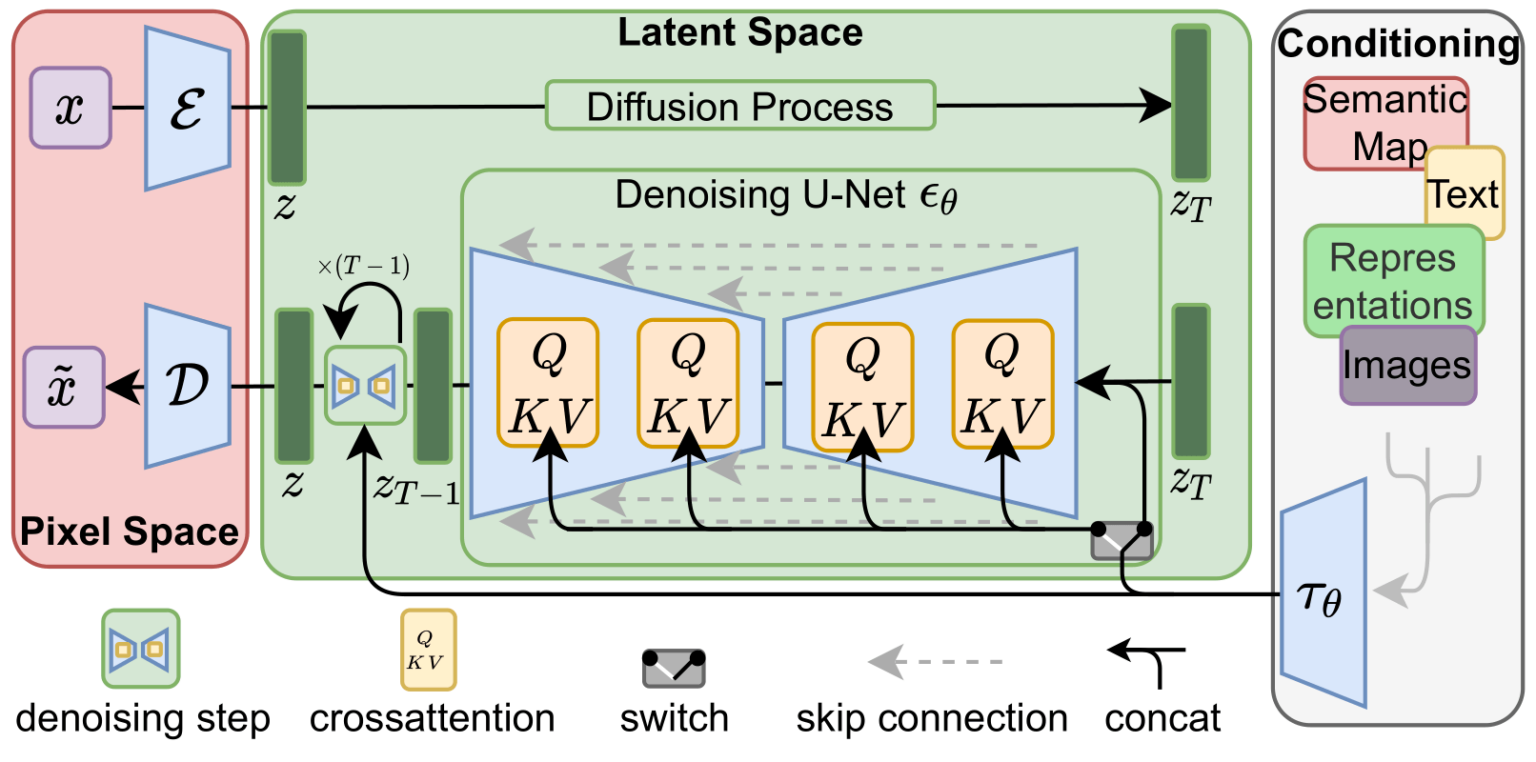
\includegraphics[width=1\linewidth]{article-Figure3-1-1536x762.png}
    \caption{Architectural diagram of a conditional diffusion model. The system operates between Pixel Space (left) and Latent Space (center), with various conditioning inputs (right). The process begins with an encoder ($\epsilon$) mapping input images ($x$) to latent representations ($z$), followed by a forward diffusion process reaching noise level $z_T$. The denoising phase employs a U-Net ($\epsilon_\theta$) with cross-attention mechanisms ($Q$,$K$,$V$) that incorporate conditioning signals ($\tau_\theta$) from text, semantic maps, and other representations. The iterative denoising process transitions from $z_T$ to $z_{T-1}$ and continues until reaching $z$, after which the decoder ($\mathcal{D}$) reconstructs the output image ($\tilde{x}$). Skip connections (dashed arrows) facilitate information flow across the U-Net, while the concatenation operations (black arrows with T-junctions) integrate features at multiple scales.}
    \label{fig:diffusion_architecture}
\end{figure}

\subsection*{1. Denoising Diffusion Probabilistic Models (DDPM)}
\begin{itemize}
  \item \textbf{Generative process:}  
    \begin{itemize}
      \item Forward: add Gaussian noise in $T$ small steps to a clean image $x_0$, producing noisy $x_t$.  
      \item Reverse: learn a denoiser $\varepsilon_\theta(x_t,t)$ to recover $x_{t-1}$ from $x_t$.  
      \item Objective: minimize 
        \[
          \mathcal{L}_{\text{DDPM}} = \mathbb{E}_{x,\varepsilon\sim\mathcal{N}(0,1),t}\bigl[\|\varepsilon - \varepsilon_\theta(x_t,t)\|^2\bigr].
        \]
    \end{itemize}
  \item \textbf{Drawbacks:}
    \begin{itemize}
      \item Operates in high-dimensional \emph{pixel} space, so each sampling step requires a full UNet pass on the full image.
      \item Typically uses hundreds to thousands of timesteps: inference is slow (e.g.\ 50 K samples take ~5 days on A100) and training can cost \(\sim\)150–1000 V100-GPU-days.
      \item Requires large datasets to learn pixel-space noise-removal.
    \end{itemize}
\end{itemize}

\subsection*{2. Stable Diffusion (Latent Diffusion Model, LDM)}
\begin{itemize}
  \item \textbf{Key idea:} Perform diffusion not in pixels but in a learned \emph{latent} space of a powerful autoencoder.  
  \item \textbf{Two-stage training:}
    \begin{enumerate}
      \item \emph{Perceptual compression stage:}  
        Train an autoencoder $(E,D)$ (with a small KL- or VQ-regularization) to map $x\!\in\!\mathbb{R}^{H\times W\times3}$ to $z\!\in\!\mathbb{R}^{h\times w\times c}$, where $h=H/f$ (e.g.\ $f=4$).
      \item \emph{Latent diffusion stage:}  
        Train a time-conditional UNet $\varepsilon_\theta(z_t,t)$ to denoise $z_t$ back to $z_{t-1}$, minimizing
        \[
          \mathcal{L}_{\mathrm{LDM}} 
          = \mathbb{E}_{z,\varepsilon,t}\bigl[\|\varepsilon - \varepsilon_\theta(z_t,t)\|^2\bigr]
        \]
        where $z_0=E(x)$ and $z_t$ follows the fixed forward diffusion in latent space.
    \end{enumerate}
  \item \textbf{Efficiency gains:}
    \begin{itemize}
      \item Latent dimensionality is much lower ($h\!\times\!w\!\ll\!H\!\times\!W$), so each denoising step is far cheaper.
      \item Overall training and sampling speed can improve by \(\sim\!3\times\) or more compared to a pixel DDPM .
    \end{itemize}
  \item \textbf{Conditional generation:}
    \begin{itemize}
      \item Incorporate arbitrary conditioning (e.g.\ text) via a domain encoder $\tau_\phi(y)$ plus cross-attention layers in the UNet backbone
      \item At inference: use classifier-free guidance to trade off fidelity vs.\ adherence to $y$.
    \end{itemize}
  \item \textbf{Decoding:} After denoising to $\hat z_0$, reconstruct $\hat x = D(\hat z_0)$.
\end{itemize}

\subsection*{3. Main Differences DDPM vs.\ Stable Diffusion}
\begin{itemize}
  \item \textbf{Operational domain:}  
    DDPM acts on full RGB pixels; SD acts on compressed latents.  
  \item \textbf{Compute \& memory:}  
    DDPM: high FLOPs/GPU memory per step (full image).  
    SD: lower cost per step (small latent), faster sampling & training.
  \item \textbf{Model structure:}  
    DDPM = single UNet over pixels.  
    SD = (pretrained autoencoder) + latent UNet + optional text encoder + cross-attention.
  \item \textbf{Flexibility:}  
    SD reuses one autoencoder for many tasks, and its cross-attention easily supports multi-modal conditioning (text, layouts, masks), whereas DDPMs typically use simple concatenation or class conditioning.
  \item \textbf{Quality vs.\ efficiency trade-off:}  
    SD finds a near-optimal balance between compression and detail preservation by choosing $f$ (often $4$–$8$) .
\end{itemize}

\subsection*{1. Comparing Stable Diffusion (SD) vs.\ SDXL}
\begin{itemize}
  \item \textbf{Overall pipeline:} Both SD and SDXL are Latent Diffusion Models (LDMs) that operate in a compressed latent space via a pretrained VAE $(E,D)$, apply a time-conditional UNet for denoising, then decode back to pixel space.  
  \item \textbf{UNet backbone size:}  
    \begin{itemize}
      \item \emph{SD (v1.4/2.1)}: $\sim$1 B parameters in the U-Net denoiser.  
      \item \emph{SDXL 1.0}: a \emph{three times larger} UNet backbone (≈3.5 B parameters), achieved by adding more attention blocks and increasing the hidden dimensionality }.
    \end{itemize}
  \item \textbf{Text conditioning:}
    \begin{itemize}
      \item \emph{SD}: single CLIP-style text encoder, cross-attention at each UNet layer.  
      \item \emph{SDXL}: \emph{two} text encoders (e.g.\ OpenCLIP-ViT/G & CLIP-ViT/L), allowing dual-prompt or more expressive guidance; cross-attention uses the concatenated context from both encoders.
    \end{itemize}
  \item \textbf{Aspect ratios \& resolutions:}
    \begin{itemize}
      \item \emph{SD}: trained primarily at square 512×512 (later 768×768) resolutions.  
      \item \emph{SDXL}: trained on \emph{multiple aspect ratios} (e.g.\ 1:1, 3:2, 2:3, 1:2, 2:1) to retain fidelity across portrait/landscape formats .
    \end{itemize}
  \item \textbf{Refinement stage:}  
    \begin{itemize}
      \item \emph{SD}: single diffusion denoiser.  
      \item \emph{SDXL}: includes an \emph{optional refiner} UNet, applied post-hoc in an img2img fashion to sharpen and add fine details to the base SDXL .
    \end{itemize}
  \item \textbf{Sampling efficiency:}  
    \begin{itemize}
      \item Larger models slow down per-step inference, but SDXL’s improved capacity often requires fewer steps for equivalent or better quality.  
      \item A distilled “XL Turbo” variant further reduces the number of denoising steps needed.
    \end{itemize}
\end{itemize}

\subsection*{2. Explanation of the Stable Diffusion Pipeline Diagram}
A canonical SD diagram (cf.\ Fig.~\ref{fig:sd_pipeline}) breaks down into:
\begin{enumerate}
  \item \textbf{VAE Stage:}  
    \begin{itemize}
      \item \emph{Encoder $E$:} maps pixel image $x\in\mathbb{R}^{H\times W\times3}$ to latent $z=E(x)\in\mathbb{R}^{h\times w\times c}$.  
      \item \emph{Decoder $D$:} reconstructs $\tilde x=D(z)$ for training the VAE; frozen at diffusion-training time.
    \end{itemize}
  \item \textbf{Forward diffusion (latent):}  
    \[
      z_t \;=\;\sqrt{\bar\alpha_t}\,z_{t-1}\;+\;\sqrt{1-\bar\alpha_t}\,\epsilon,\quad \epsilon\!\sim\!\mathcal{N}(0,I),
    \]
    gradually corrupting $z$ with Gaussian noise over $T$ timesteps.
  \item \textbf{Denoising UNet $\varepsilon_\theta(z_t,t,y)$:}  
    \begin{itemize}
      \item \emph{Time embedding} encodes $t$.  
      \item \emph{Cross-attention} layers inject conditioning (text embeddings or other) into intermediate UNet blocks.  
      \item \emph{Skip connections} shuttle high-resolution details from encoder to decoder paths.  
      \item Predicts noise estimate $\hat\epsilon$ to recover $z_{t-1}$ from $z_t$.
    \end{itemize}
  \item \textbf{Reverse diffusion sampling:}  
    Iteratively apply the learned denoiser, optionally with classifier-free guidance, to obtain $\hat z_0$.
  \item \textbf{Reconstruction:}  
    Decode $\hat z_0$ back to pixel space: $\hat x = D(\hat z_0)$, yielding the final generated image.
\end{enumerate}
